\chapter{Introducción}

La ciencia de ondas gravitacionales es un área que vivió un rápido crecimiento en las últimas décadas. Este crecimiento llevó en septiembre del 2015 a la increíble primera detección obtenida de ondas gravitacionales producto de una colisión binaria de agujeros negros \cite{https://doi.org/10.48550/arxiv.1607.05251, LIGOScientific:2016aoc}. Actualmente los interferometros LIGO, VIRGO y KAGRA van detectando cerca de 50 eventos, y planean empezar la cuarta serie de observaciones O4 a mediados de mayo de 2023 \footnote{https://observing.docs.ligo.org/plan/}. 

Cada observación no es solo una confirmación de una de las predicciones más relevantes de las ecuaciones de Einstein, sino que pueden aportan una gran cantidad de información de los fenómenos que las producen. De una onda producida por la colisión de dos agujeros negros se pueden inferir un total de 15 parámetros, de los cuales algunos son \textit{intrínsecos} (como la relación entre las masas, o los espínes) y otros \textit{extrínsecos} (la distancia del evento, la posición en el cielo, etc) \cite{Veitch_2015}. 

La estimación de parámetros se realiza utilizando inferencia Bayesiana \cite{Thrane_2019}, un método que requiere generar funciones de onda para diversos parámetros en tiempo real. Esto es un problema debido a la dificultad que representa el resolver las ecuaciones de Einstein; para obtener la función de onda producto de una colisión binaria utilizando relatividad numérica se necesitan meses de cómputo. Debido a que se necesitan varias configuraciones al momento de realizar la inferencia de parámetros, la relatividad numérica no es una opción a la hora de generar las funciones de onda. En esta tésis se trabajará dentro del marco de los modelos sustitutos \cite{Field_2014}, una alternativa que logra generar resultados de alta precisión, comparable a aquella de los métodos de relatividad numérica, pero en tiempo real y en una simple computadora portátil.

La construcción de un modelo sustituto de orden reducido se puede explicar a grandes rasgos en tres etapas: 1) se seleccionan $n$ configuraciones dentro de un dominio de parámetros para representar a todo el dominio, 2) se realiza una interpolación en el dominio temporal, 3) se vuelve a realizar una interpolación, pero esta vez en el espacio de los parámetros. Como resultado se obtiene un modelo predictivo capaz de generar resultados precisos y en tiempo real (este proceso está explicado en la siguiente review \cite{Tiglio:2021ysj}).

Si bien el objetivo final es crear un modelo predictivo, este trabajo se centra solo en la primera parte de la construcción del modelo; la representación. Esto se logra utilizando bases reducidas \cite{rb0book, doi:10.1137/09075250X, PhysRevLett.106.221102, 10.1115/1.1448332, rb1book} construidas a partir de un algoritmo voraz o \textit{greedy}. Este método busca eliminar la redundancia que pueda estar presente en un conjunto de soluciones para un dado espacio de parámetros, de forma que se logre representar todo el espacio a partir de un número relativamente bajo de elementos.

Para ser más precisos, este trabajo se centra en la optimización de hiperparámetros para la construcción de una base reducida con refinamiento \textit{hp-greedy} \cite{Cerino:2022dhr}. Este refinamiento divide el espacio de parámetros en distintos subdominios de forma iterativa, logrando una estructura de árbol binario. Una ventaja de esto es poder trabajar con espacios de parámetros que presenten discontinuidades, y otra es la reducción del tiempo de proyección de un espacio a la base reducida, lo que daría lugar a un modelo más rápido y eficiente. Una base reducida \textit{hp-greedy} constituye un sistema de aprendizaje supervisado con un gran número de configuraciones de hiperparámetros, las cuales afectan en gran medida el rendimiento del sistema, por lo que resulta interesante concentrarse en el problema de optimizar la construcción de este sistema. 

Un método de optimización cada vez más utilizado dentro de distintas áreas de la ciencia de datos es la optimización Bayesiana \cite{7352306, https://doi.org/10.48550/arxiv.1012.2599}, con resultados sobresalientes a la hora de entrenar distintos modelos de aprendizaje automático y aprendizaje profundo. 
Realizar una elección manual de los hiperparámetros de una base reducida \textit{hp-greedy} lleva a resultados mediocres en general, por lo que es necesario realizar muchas pruebas antes de encontrar una mejora con respecto al resultado inicial. La optimización Bayesiana es una forma de automatizar este proceso a la vez que cada nueva evaluación será una elección informada a partir de las evaluaciones realizadas anteriormente. Por esta razón se optó por utilizar la optimización bayesiana, obteniendo resultados bastante favorables para minimizar de máximmo error de representación de las bases construidas.






%En esta tésis se buscó optimizar un sistema de aprendizaje supervisado entrenado para lograr una representación compacta de ondas gravitacionales utilizando bases reducidas \cite{rb0book, doi:10.1137/09075250X, PhysRevLett.106.221102, 10.1115/1.1448332, rb1book}, con el fin de facilitar esta inferencia de parámetros. En este capítulo se hablará de la motivación y el objetivo detrás de este trabajo. Luego se dará una breve introducción a la representación de ondas gravitacionales y por último se explicará de dónde provienen los datos utilizados. 






%Desde la primera observación directa de ondas gravitacionales y primera observación de una colisión binaria de agujeros negros\cite{LIGOScientific:2016aoc}

%modelado de orden reducido \cite{Field_2014}
 %review\cite{Tiglio:2021ysj} 
 
 %Bases Reducidas \cite{rb0book, doi:10.1137/09075250X, PhysRevLett.106.221102, 10.1115/1.1448332, rb1book}

% ciencia de ondas grav \cite{https://doi.org/10.48550/arxiv.1607.05251}

%est. param \cite{Veitch_2015}

\newpage


\section{Representación Ondas Gravitacionales}

ondas grav. rel num \cite{Centrella_2010}
\section{Datos utilizados}

Se utilizaron ondas gravitacionales generadas a partir del modelo híbrido \textit{NRHybSur3dq8}\cite{Varma_2019} de relativdad numérica y aproximaciones post Newtonianas para colisiones de agujeros negros binarios.
\\

Cada onda \(h\) generada se representa por una serie temporal compleja de la forma:
\[
h = h_+ + ih_{\times}
\]


Recordando que $h$ está parametrizada por \(\lambda\)

 \[h = h(t; \lambda) = h_{\lambda}(t) = h_{\lambda} \]
 
En este caso \(\lambda\) tendrá 3 dimensiones, $(q, \chi_{1_Z},\chi_{2_Z}) $, y estará acotado de la siguiente manera:

\begin{itemize}
\item Relación entre masas $q$: $1 \le q \le 8$
\item Espín del agujero negro más pesado (liviano) $\chi_{1_Z} (\chi_{1_Z})$: $|\chi_{1_Z}|, |\chi_{2_Z}| < 0.8$
\end{itemize}

\begin{figure}[h]
\centering
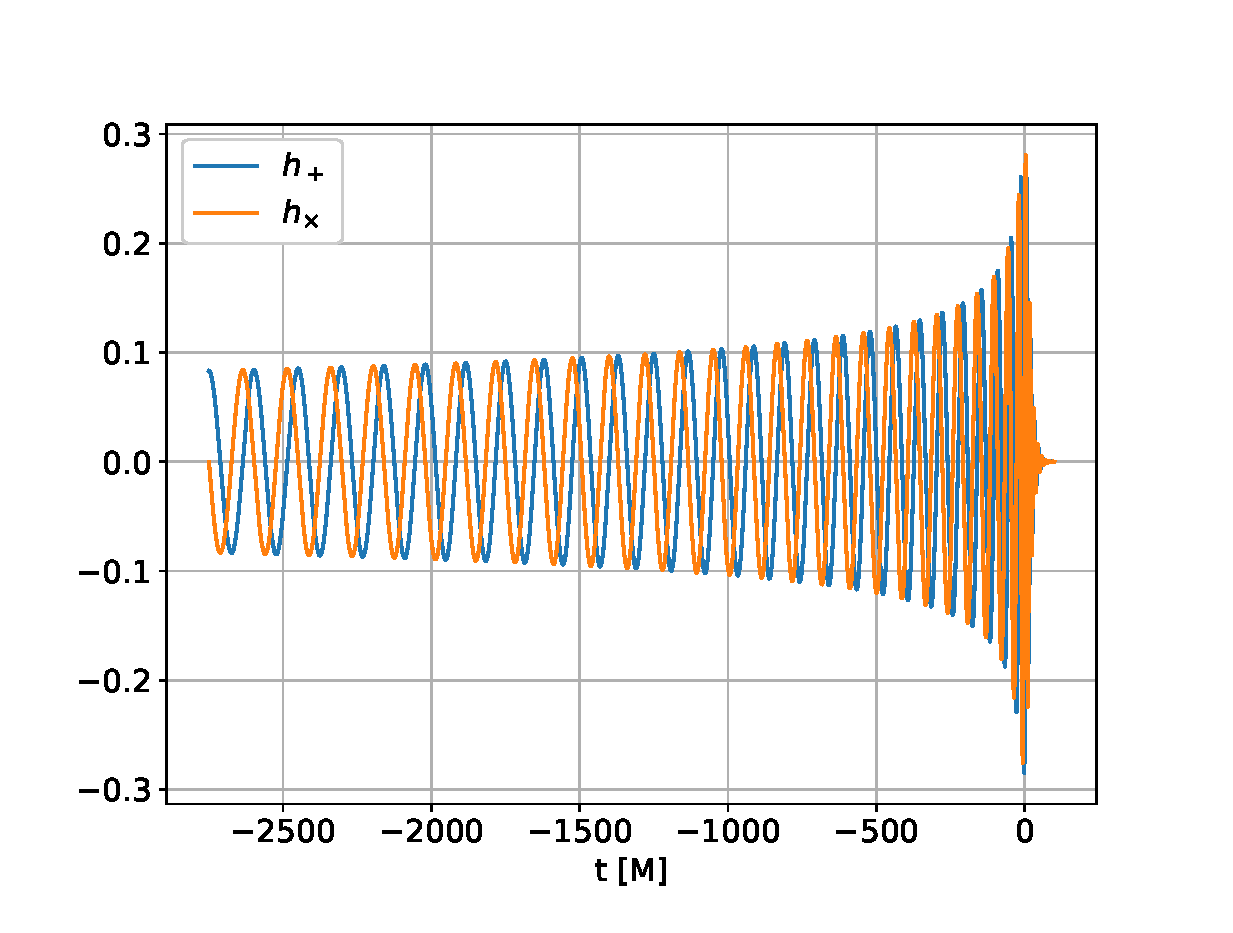
\includegraphics[width=.9\columnwidth]{figs/h_l2m2_q3.eps}
\caption{polarizaciones \(h_+\) y \(h_{\times}\) para $q = 3$, $\chi_{1_Z} = \chi_{2_Z} = 0$, en el modo $l=2$, $m=2$.}
\label{fig:h_q3}
\end{figure}



Se representa un conjunto \( \mathcal{K} \) de N muestras de $\lambda$ de la siguiente forma:

\[ \mathcal{K}  = \{h_{\lambda_i}\}, \hspace{5mm} i = 1, ..., N\]

y debido a que cada $h_{\lambda_i}$ es una serie temporal, se puede representar $\mathcal{K}$ en forma de la matriz $H \in \mathbb{C}^{N\times L}$:

\[
H = 
\begin{bmatrix}
h_{\lambda_1} \\
h_{\lambda_2} \\
 \vdots \\
 h_{\lambda_N} \\
\end{bmatrix}
= 
\begin{bmatrix}
h_{\lambda_1}(t_1) & h_{\lambda_1}(t_2)  & \cdots & h_{\lambda_1}(t_L)\\
 h_{\lambda_2}(t_1) & h_{\lambda_2}(t_2)  & \cdots & h_{\lambda_2}(t_L)\\
 \vdots & \vdots & \ddots &  \vdots \\
h_{\lambda_N}(t_1) & h_{\lambda_N}(t_2)  & \cdots & h_{\lambda_N}(t_L)
\end{bmatrix}
\]

Siendo $L$ la longitud de la serie temporal. De forma que cada fila de $H$ es una onda gravitacional.


% Por las citas nomas:

%\cite{Pinkus1985nWidthsIA}:
%Por lo tanto $d_n$ sirve como un límite superior; es lo mejor que se puede lograr si la base fue escogida de forma óptima.
%En algunos casos $d_n$ se puede calcular teóricamente \cite{MAGARILILYAEV200197}. Más específicamente se puede probar que $d_n \sim n^{-r}$ para funciones con sus primeras $(r-1)$ derivadas continuas y que $d_n \sim e^{-an^b}$ para funciones con una dependencia $C^{\infty}$  \cite{articleg}. En el contexto de ondas gravitacionales se espera un comportamiento asíntotico de convergencia exponencial con $n$ %\citep{PhysRevX.4.031006, Herrmann:2012xpx}.
%\cite{https://doi.org/10.48550/arxiv.1204.2290}
%\cite{Caudill_2012}